%% ----------------------------------------------------------------
%% Thesis.tex -- MAIN FILE (the one that you compile with LaTeX)
%% ---------------------------------------------------------------- 

% Set up the document
\documentclass[a4paper, 11pt, oneside]{Thesis}  % Use the "Thesis" style, based on the ECS Thesis style by Steve Gunn
\graphicspath{Figures/}  % Location of the graphics files (set up for graphics to be in PDF format)

% Include any extra LaTeX packages required
\usepackage[square, numbers, comma, sort&compress]{natbib}  % Use the "Natbib" style for the references in the Bibliography
\usepackage{verbatim}  % Needed for the "comment" environment to make LaTeX comments
\usepackage{vector}  % Allows "\bvec{}" and "\buvec{}" for "blackboard" style bold vectors in maths
\usepackage{array}
\usepackage{booktabs}
\usepackage{arydshln}
\usepackage{filecontents}
\usepackage[threshold=1]{csquotes}  
%\usepackage{graphicx}
\usepackage[table]{xcolor}
\newcolumntype{?}{!{\vrule width 2pt}}

\hypersetup{urlcolor=blue, colorlinks=true}  % Colours hyperlinks in blue, but this can be distracting if there are many links.

%% ----------------------------------------------------------------
\begin{document}
\frontmatter      % Begin Roman style (i, ii, iii, iv...) page numbering

% Set up the Title Page
\title  {The expected shape of the Milky Way's dark matter halo}
\authors  {\texorpdfstring
            {\href{https://github.com/jdprada1760}{Jesus David Prada Gonzalez}}
            {Jesus David Prada Gonzalez}
            }
\addresses  {\groupname\\\deptname\\\univname}  % Do not change this here, instead these must be set in the "Thesis.cls" file, please look through it instead
\date       {\today}
\subject    {}
\keywords   {}

\maketitle
%% ----------------------------------------------------------------

\setstretch{1.3}  % It is better to have smaller font and larger line spacing than the other way round

% Define the page headers using the FancyHdr package and set up for one-sided printing
\fancyhead{}  % Clears all page headers and footers
\rhead{\thepage}  % Sets the right side header to show the page number
\lhead{}  % Clears the left side page header

\pagestyle{plain}  % Finally, use the "fancy" page style to implement the FancyHdr headers

%% ----------------------------------------------------------------
% Declaration Page required for the Thesis, your institution may give you a different text to place here
%\Declaration{
%
%\addtocontents{toc}{\vspace{1em}}  % Add a gap in the Contents, for aesthetics
%
%I, AUTHOR NAME, declare that this thesis titled, `THESIS TITLE' and the work presented in it are my own. I confirm that:
%
%\begin{itemize} 
%\item[\tiny{$\blacksquare$}] This work was done wholly or mainly while in candidature for a research degree at this University.
% 
%\item[\tiny{$\blacksquare$}] Where any part of this thesis has previously been submitted for a degree or any other qualification at this University or any other institution, this has been clearly stated.
% 
%\item[\tiny{$\blacksquare$}] Where I have consulted the published work of others, this is always clearly attributed.
% 
%\item[\tiny{$\blacksquare$}] Where I have quoted from the work of others, the source is always given. With the exception of such quotations, this thesis is entirely my own work.
% 
%\item[\tiny{$\blacksquare$}] I have acknowledged all main sources of help.
% 
%\item[\tiny{$\blacksquare$}] Where the thesis is based on work done by myself jointly with others, I have made clear exactly what was done by others and what I have contributed myself.
%\\
%\end{itemize}
% 
% 
%Signed:\\
%\rule[1em]{25em}{0.5pt}  % This prints a line for the signature
% 
%Date:\\
%\rule[1em]{25em}{0.5pt}  % This prints a line to write the date
%}
%\clearpage  % Declaration ended, now start a new page

%% ----------------------------------------------------------------
%% The "Funny Quote Page"
%\pagestyle{empty}  % No headers or footers for the following pages
%
%\null\vfill
%% Now comes the "Funny Quote", written in italics
%\textit{``Write a funny quote here.''}
%
%\begin{flushright}
%If the quote is taken from someone, their name goes here
%\end{flushright}
%
%\vfill\vfill\vfill\vfill\vfill\vfill\null
%\clearpage  % Funny Quote page ended, start a new page
%% ----------------------------------------------------------------

% The Abstract Page
\addtotoc{Abstract}  % Add the "Abstract" page entry to the Contents
\abstract{
\addtocontents{toc}{\vspace{1em}}  % Add a gap in the Contents, for aesthetics
The shape of the Dark Matter (DM) structure (halo) in which a galaxy is embedded is heavily determined by the anisotropic accretion of mass from its specific environment. Therefore, the shape of a galaxy's halo is an important feature to inquire about its formation history and the relation of DM and gas within it. In this work we study the shape of the DM halo of Milky Way-like galaxies from the Auriga simulations. We focus on the radial and time dependence. We found that, on DM-only and Magneto-hydrodynamic (MHD) simulations, the shape of the DM halo is more triaxial in the inner-skirts than in the outter-skirts. We compared simulations with and without gas and verified that the presence of visible matter has an effect of rounding the DM halo which is amplified for smaller radii, where the gravitational potential of the galactic disk becomes more significant. Regarding the effect of time on the DM halo shape, we corroborated that it is well-conserved in comoving units until $z \approx 2$. This means that probing the halo shape at the virial radius in physical units for different redshifts is nearly equivalent to probing the shape at different radii at redshift $0$. These results are in accordance with previous work on cosmological and galactic-size simulations, and may serve as guidelines to improve observational constraints on our MW DM halo.
}

\clearpage  % Abstract ended, start a new page

% The Abstract Page
\addtotoc{Resumen}  % Add the "Abstract" page entry to the Contents
\abstract{
\addtocontents{toc}{\vspace{1em}}  % Add a gap in the Contents, for aesthetics
La forma de la estructura (halo) de Materia Oscura en la cual est\'a embebida una galaxia es altamente determinada por la acreci\'on anisotr\'opica de materia en el entorno espec\'ifico en el que \'esta se encuentra. Es por esto que la forma del halo de una galaxia es una caracter\'istica imporatnte para indagar sobre su historia de formaci\'on y la relaci\'on entre Materia Oscura y gas dentro de ella. En este trabajo estudiamos la forma de los halos de materia oscura en galaxias de tipo V\'ia L\'actea del cat\'alogo de simulaciones Auriga. Nos centramos principalmente en su dependencia radial y temporal. Hemos encontrado, en simulaciones de s\'olo Materia Oscura y en simulaciones de Magneto-hidrodin\'amica, que la forma del halo es m\'as triaxial en las partes de adentro que en las afueras. Al comparar simulaciones con y sin gas, verificamos que la presencia de materia visible tiene un efecto de redondeado sobre el halo de Materia oscura, el cual es amplificado en radios peque\~nos, donde el efecto gravitacional del disco gal\'actico se torna significante. En cuanto al efecto del tiempo en la forma del halo de Materia Oscura, hemos corroborado que esta se conserva en unidades com\'oviles hasta $z \approx 2$. Esto se ve reflejado en la aproximada equivalencia entre el muestreo de la forma en el radio virial en unidades f\'isicas a diferentes redshifts y el muestreo a diferentes radios en la actualidad. Estos resultados son respaldados por trabajos previos en simulaciones de escala gal\'actica y cosmol\'ogica, y pueden servir como lineamientos para mejorar las mediciones de la forma del halo de Materia Oscura de nuestra V\'ia L\'actea. 

}
\clearpage  % Abstract ended, start a new page

%% ----------------------------------------------------------------

%% The Abstract Page
%\addtotoc{Abstract MOCCA}  % Add the "Abstract" page entry to the Contents
%\abstract{
%\addtocontents{toc}{\vspace{1em}}  % Add a gap in the Contents, for aesthetics
%Given the elusive nature of Dark Matter (DM), indirect measurements are the most common approach to study it observationally. However, to make these studies possible, some assumptions must be made. These assumptions come from complicated theoretical frameworks and the analysis of state-of-the-art cosmolofical simulations. In this work we study the shape of the DM halo of Milky Way-like galaxies from the Auriga simulations. We focus on the radial and time dependence. We found that, on DM-only and Magneto-hydrodynamic (MHD) simulations, the shape of the DM halo is more triaxial in the inner-skirts than in the outter-skirts. We compared simulations with and without gas and verified that the presence of visible matter has an effect of rounding the DM halo which is amplified for smaller radii, where the gravitational potential of the galactic disk becomes more significant. Regarding the effect of time on the DM halo shape, we corroborated that it is well-conserved in comoving units until $z \approx 2$. This means that probing the halo shape in physical units at the virial radius for different redshifts is nearly equivalent to probing the shape at different radii at redshift $0$. These results are in accordance with previous work on cosmological and galactic-size simulations, and may serve as guidelines to improve observational constraints on our MW DM halo.
%}
%
%\clearpage  % Abstract ended, start a new page
%% ----------------------------------------------------------------

\setstretch{1.3}  % Reset the line-spacing to 1.3 for body text (if it has changed)

% The Acknowledgements page, for thanking everyone
\acknowledgements{
\addtocontents{toc}{\vspace{1em}}  % Add a gap in the Contents, for aesthetics

I am grateful with my mother and brother who encouraged me to work hard and cheered me up in difficult moments. I am also truly thankful with my advisor Jaime Forero for all the doors he has opened for me and for being my scientific father. I express my gratitude to my dad, without whom my Physics career would not have been possible.\ldots


}
\clearpage  % End of the Acknowledgements
%% ----------------------------------------------------------------

\pagestyle{fancy}  %The page style headers have been "empty" all this time, now use the "fancy" headers as defined before to bring them back


%% ----------------------------------------------------------------
\lhead{\emph{Contents}}  % Set the left side page header to "Contents"
\tableofcontents  % Write out the Table of Contents

%% ----------------------------------------------------------------
\lhead{\emph{List of Figures}}  % Set the left side page header to "List if Figures"
\listoffigures  % Write out the List of Figures

%% ----------------------------------------------------------------
\lhead{\emph{List of Tables}}  % Set the left side page header to "List of Tables"
\listoftables  % Write out the List of Tables

%% ----------------------------------------------------------------
%\setstretch{1.5}  % Set the line spacing to 1.5, this makes the following tables easier to read
%\clearpage  % Start a new page
%\lhead{\emph{Abbreviations}}  % Set the left side page header to "Abbreviations"
%\listofsymbols{ll}  % Include a list of Abbreviations (a table of two columns)
%{
%% \textbf{Acronym} & \textbf{W}hat (it) \textbf{S}tands \textbf{F}or \\
%\textbf{LAH} & \textbf{L}ist \textbf{A}bbreviations \textbf{H}ere \\
%
%}

%% ----------------------------------------------------------------
%\clearpage  % Start a new page
%\lhead{\emph{Physical Constants}}  % Set the left side page header to "Physical Constants"
%\listofconstants{lrcl}  % Include a list of Physical Constants (a four column table)
%{
%% Constant Name & Symbol & = & Constant Value (with units) \\
%Speed of Light & $c$ & $=$ & $2.997\ 924\ 58\times10^{8}\ \mbox{ms}^{-\mbox{s}}$ (exact)\\
%
%}

%% ----------------------------------------------------------------
%\clearpage  %Start a new page
%\lhead{\emph{Symbols}}  % Set the left side page header to "Symbols"
%\listofnomenclature{lll}  % Include a list of Symbols (a three column table)
%{
%% symbol & name & unit \\
%$a$ & distance & m \\
%$P$ & power & W (Js$^{-1}$) \\
%& & \\ % Gap to separate the Roman symbols from the Greek
%$\omega$ & angular frequency & rads$^{-1}$ \\
%}
%% ----------------------------------------------------------------
% End of the pre-able, contents and lists of things
% Begin the Dedication page

\setstretch{1.3}  % Return the line spacing back to 1.3

\pagestyle{empty}  % Page style needs to be empty for this page
\dedicatory{Dedicated To my Mother and my little brother\ldots}

\addtocontents{toc}{\vspace{2em}}  % Add a gap in the Contents, for aesthetics


%% ----------------------------------------------------------------
\mainmatter	  % Begin normal, numeric (1,2,3...) page numbering
\pagestyle{fancy}  % Return the page headers back to the "fancy" style

% Include the chapters of the thesis, as separate files
% Just uncomment the lines as you write the chapters

\chapter{Introduction}

\section{About Dark Matter}

In the field of observational astronomy it is very plausible to encounter ourselves with indirect or direct measurements which are not reconcilable with the current understanding of physical theories. Very often, these intriguing measurements are the result of inaccuracy in the measurement device or the asumption of some erroneous or non-precise premises. However, since the early beginings of the 20th century, we have found inconsistencies of observations with the accepted paradigm of physics, which have been reliably proven not to arise from any errors in the premises or devices. These inconsistent measurements principally question the veracity of the Newtionan gravity or even its improved Einstenian version at astronomical and cosmological scales.\\

The principal problem of these inconsistencies can be resumed to the fact that we observe that objects are moving in a certain way that cannot be explained exclusively by the effect of gravitational forces of visible matter. In fact, there is very strong historical evidence that this gravitational effect is heavily \textit{underestimated} if we only take into account the effect of light-interacting matter. To solve this problem without blaming the measurement instruments or the used premises, which have been consistently ruled out as the sources of these discrepancies, there are two important hypothesis to study.\\

One of these hypothesis, which is the most simple to understand, tries to reconcile these observations with Newtonian gravity, or even more, General Relativity, assuming it is completely valid in the cosmological context. Consequently, if there is nothing wrong with the theoretical framework, the premises, nor the instruments, and gravitational effects cannot be explained solely with the matter that we observe, then there must exist some kind of matter that exerts this missing gravitational pull, which we cannot see for some reason. We talk about Dark Matter (DM).\\

Since early as the 1930's, the DM hypothesis has been considered. It is known that Fritz Zwicky proposed the presence of some kind of DM within the Coma cluster of galaxies to explain the cluster attachment despite the galaxie's huge velocities that would have made them scape \cite{Fritz}. At first, this proposal was not given much attention as there were many other sources of errors to blame, and these observations were not widely replicated. Nevertheless, as years passed, more and more inconsistencies could be explained with the use of this DM hypothesis. It is the case of the famous rotation curves \cite{rotationCurves} where the ammount of visible matter on galaxies could not account for the centripetal acceleration associated with the tangential velocities of stars within a it. It is, in essence, the argument of Zwicky. Later on, with a better understanding of the space-curving effect of matter predicted by general relativity and the improvement of precision in telescopes, it was posible to measure weak lensing (gravitational distortion of observed objects) through massive clusters of galaxies \cite{weak_Lensing}. Again, this effect was estimated to be much more dim compared to the actual result of observations, suggesting the existence of DM. This is, in fact, a naturally different approach than those of velocity-curves analysis.\\

Less direct evidence of DM include arguments related to structure formation and the observed Cosmig Microwave Background Radiation (CMBR) \cite{structure formation}. On one hand, the structure formation argument is based in the fact that the early stages of the universe were dominated by radiation, which heavily affects visible matter by preventing it to grow clumps from small density anisotropies. In fact, the speed of sound at the early stages of the universe is very close to that of the speed of light, meaning that density anisotropies must be quite large and localized for them to not be dispersed as sound waves. These anisotropies would be evidenced on the CMBR as temperature fluctuations. It has been thoroughly corroborated that these anisotropies are not present on a very precise sampling of the CMBR like WMAP \cite{WMAP} and PLANCK \cite{PLANCK} In the absence of any other kind of pulling force or sort of matter with smaller speed of sound, such as DM, we would not have the same distribution of collapsed structures we observe today, like stars, galaxies, clusters, etc. as these density fluctuations would have been dispersed. \\


Subsequently, the second important hypothesis to reconcile observations with our theoretical framework is of oposing nature than that of DM. In this case, we study the posibility that there General Theory of Relativity is not accurate and is in fact underestimated at cosmological scales. We talk in this case of Modified-Newtonian Dynamical (MOND) theories. This is a natural consequence of assuming that the universe is what we observe and there is no such thing as non-visible matter. If we apply this hypothesis to the problems solved with the assumption of the existence of DM, under a precise tunning of parameters of these new theories, we could obtain the seeked consistency. However, the problem arises when we try to satisfy this consistency for all observational discrepancies. In the case of DM, many of the observational mismatches with theory may be solved and it is possible to make predictions. In the case of MOND theories, many results as rotation curves may be emulated to certain extent \cite{MOND}, but given its strong claims, it is some times imposible to reconcile with observations \cite{MOND NO}. In fact, these teories are extremely well constrained for small-scale regimes, which restricts the freedom with which this models may be adjusted to observations, to such an extent that some times a remanent of DM is needed to completely concile the theory with observation \cite{DM remanent.}.\\

For these reasons, DM is the most widely accepted hypothesis to account for these observational discrepancies. Nonetheless, a complete physical picture of DM is still missing and it is one of the biggest puzzles to fully understand the composition of our Universe. Many appealing candidates may be found in the context of Particle Physics, which motivate the existence different kinds of weak-interacting particles through interesting symmetry-seeking theories \cite{particle physics.}.\\

\section{Theoretical background for DM}


\section{Constraining the Milky Way's DM Halo}
So far, DM presence can only be measured through its gravitational effect on the surrounding visible matter. 
One of best the astronomical systems that can be used to probe DM on astronomical scales is our own galaxy: the Milky Way (MW).
Probing the DM density field around our galaxy (it's so-called DM halo) can shed light on the nature of DM \cite{Nipoti,ReadMoore} and our
galaxy's formation history \cite{Read1,Read2,Vera-Ciro2011}.\\

DM haloes have two important features that could be constrained. 
On one hand there is the density profile, which has been demonstrated to follow an approximately universal model \cite{Navarro et al. 2010}. 
On the other hand, there is the halo shape, which is directly related to its spin. 
According to the hierarchical model of structure formation, due to the anisotropic history of accretion DM haloes are triaxial and therefore, their shape and spin are important characteristics to \textbf{diagnose} their formation history \cite{Bardeen et al. 1986}.\\

In this sense, it is of special interest to constrain the DM halo shape of the only cosmological object of which we have a tridimensional view from inside: our Milky Way. However, this is a very difficult labour given the observational restrictions of observation. Many approaches have been made to constrain the MW's DM shape. One of them is to make use of theoretical models that relate the content of matter of our galaxy with the gravitational potential.\\

For example, Loebman et al. \cite{Loebman et al 2012} used the axisymmetric Jean's equations \cite{Jean 2015} that relate the stellar content of our galaxy, with the radial and axial accelerations. 
The observed accelerations cannot be completely explained by visible matter only and DM presence is needed. Loebman et al. estimated that, around 20Kpc, the DM halo must be perfectly oblate with axis ratio of $q_{DM}=0.47 \pm 0.14$ to account for this discrepancy.\\

Nevertheless, the axial symmetry that characterizes this halo is inherited from the use of axisymmetric Jean's equations. 
Although this is a strong asumption, a more general theoretical background is much more difficult to implement given the difficulty to obtain the needed data from observations. 
Even authors aknowledge that "... while it is premature to declare $q_{DM}=0.47 \pm 0.14$ as a robust measurement of the dark matter halo shape, it is encouraging that the simulation is at least qualitatively consistent with SDSS data in so many aspects".
This demonstrates that this field of study is still very young and any calculated constraint may lead us to a better understanding of our MW's DM halo shape.\\

A more common and strong approach is to use the streams of close dwarf galaxies that have been deformed by the gravitational potential of the MW. 
This effect is very important because the torca generated by the anisotropy in our halo is sensible to its parameters and thus, these streams are strong evidence to constrain the shape of our MW's DM halo \cite{See Law-Majewski references}. 
In fact, it is known that a static axisymmetric halo cannot simultaneously explain all the features of the Sagittarius leading arm \textbf{citaa}. \\

In this context Law and Majewski 2010 proposed an analytical model of the MW consisting of a fixed analytical gravitational potential formed by a Miyamoto-Nagai \cite{Miyamoto-Nagai 1985} disk, a Hernquist spheroid and a logarithmic halo. 
This halo is triaxial and is characterized by its axial ratios and orientation. 
Given all these parameters, the Sagittarius stream was simulated and evolved forward and backwards in time for various choices of the halo parameters. 
The best fit, compared to a detailed study of the observational properties of the Sagittarius stream, was found at a minor/major axis ratio $(c/a)_{\Phi}=0.72$ and intermediate/major axis ratio $(b/a)_{\Phi}=0.99$. The minor axis of this triaxial halo was found to be pointing in some direction contained in the galactic disk plane. \\

This sophisticated model succeeded at simultaneously reproducing the radial velocity and angular position trends of the Sagittarius leading arm, which were troublesome to model with simpler approaches. 
Nevertheless, the coexistence of a triaxial DM halo and an axisymmetric galactic disk is not supported by Cold Dark Matter (CDM) models \cite{Debattista et al. 2008}. 
Specifically, it is expected that the DM and gas distributions are correlated in the sense that matter is accreted similarly as is DM, being the interaction properties the principal difference in the behaviour. 
Having this into account, gas and DM must have aligned angular momenta to certain extent because all kinds of matter are expected to be accreted from the same cosmic structures. 
In other words, it is expected for minor axes to be rather aligned. 
Furthermore, due to stability reasons and a historical interaction, the matter distribution should be non-axisymmetric in the presence of a non-axisymmetric halo potential.\\

Law \& Majewski comment in their paper: "... by no means do they (results) represent best-fit models in a statistical sense. Therefore, the predictions made cannot be considered exclusive or definitive but serve to guide where future observations could focus to distinguish between various models.". 
Particularly, this discrepancy with the current CDM paradigm may be a feature of the specific model. 
Other important observational constraints were dismissed in this study, such as the non-symmetric influence of the Large Magellanic Cloud (LMC). 
This feature may obviate the triaxial halo and produce a more CDM-consistent model. 
However, observationally obtaining the detailed information of the LMC needed for this kind of research is extremely difficult.\\

Studies of this kind are by nature non-conclusive(deterministic?, not so conclusive?) due to the dificulty in obtaining precise information from observations. 
In observations, we take 2-dimensional snapshots of the sky and therefore, we loose resolution of the radial density field due to screening. 
This makes the process of obtaining  a tridimensional view of a cosmological-scale object an extremely difficult endeavour. 
Furthermore, we can determine radial velocities with dopler effect, but there is no obvious way of obtaining tangencial velocities. 
Bearing this in mind, any study which is sensible to very detailed observational parameters for obtaining non-direct measurements of the DM density field will be either non-conclusive for reasonable-difficulty models (as is the process of constraining), or must be extremely sophisticated to achieve a significantly conclusive result.\\

\section{State of the art on MW simulations}
To address this specific difficulty of obtaining information from observations, there is a vast and important field consisting in the modeling of the non-linear behaviour of matter. 
This is with the objective of numerically simulating the universe at a wide range of scales and produce consistent systems of which we have  full control of their parameters at all stages. 
In this sense, a computer may become a virtual cosmological-scale laboratory, where we may run an experiment having full control over its initial conditions to compare different outputs and support theoretical frameworks. \\

In this sense, in the CDM paradigm, we have fully theoretical studies \cite{Bardeen et al. 1986,Schechter} principally focused in the analysis of Gaussian random fields and the properties of self-similarity that DM must possess. 
These theoretical frames are then supported by CDM simulations \cite{Cualquier estudio de CDM hace referencia a esos pilares} and, if possible, by observations. 
In fact, these theories are usually thoroughly verified and complemented through simulations, given their convenient malleability, before being directly applied to observations.\\ Redactar mejor (simbiosis entre teor[ia analitica, simulaciones numericas, y observaciones.

One good example of this synergy between analytical models, numerical simulations and observational data is evidenced in the work of Vera-Ciro et al. (2011-2013). In 2011, Vera-Ciro et al. studied the shape of a set of four simulated MW-like DM galaxies with the objective of complementing the predictions of the CDM paradigm. Specifically, the hierarchical model of structure formation predicts that the halo shape is correlated with the environment given that it determines the structures from which it accretes matter \cite{referencias sobre relacion entre forma y entorno}. However, theoretical studies are restricted to the correlations at reshift 0 and do not say much about history of formation. Intuitively, it is expected that halo shapes vary with the radius taking into account that accretion occurrs at progresively bigger radii in history and that the cosmic structures that determine environments evolve during that time. Due to the collisionless nature of DM, inner shells can interact with outer shells only in a gravitational way. This means that the historical shape is somewhat conserved in the radial shape profile.\\

Vera-Ciro et al.  showed in 2011 that the radial profile of the halo shape is indeed correlated with its accretion history and environment. Furthermore, due to the increase in the cross section of the halos, which contributes to the scattering of particles(?), at later stages and bigger radii, they become more oblate/spherical. This results helped to obtain more insight about the galactic dynamics of formation and also suggested some guidelines to improve Law \& Majewski 2010 study.\\

In 2013, Vera-Ciro et al. proposed an improved study based on the one by Law \& Majewski in 2011. Vera-Ciro et al. proposed a halo that is perfectly oblate at inner regions and transitions smoothly to a triaxial halo in the outter-skirts. With this, the angular momentum inconsistency of this constraint with the CDM model is solved. They found that this halo is triaxial in the outter skirts with a medium-to-major axis ratio of $0.9$ and minor-to-major axis of $0.8$, which is still very oblate regarding the CDM predictions.\\

However, even when this study solves some inconsistencies with the expected predictions, it demonstrated that small perturbations are important. That is, even when the Sagittarius stream samples the gravitational potential at the outter parts of the halo, where the shape of the inner regions should not be so important, the outter shape is affected to compensate for the change in the regions from inside. This effect takes our attention to a relegated topic: the LMC. In fact, Vera-Ciro et al. demonstrated that the change in shape from the inner regions produces a torque comparable to that of the LMC, which should be taken into account in further researches.\\

%
%Briefly talk about the work of Vera-Ciro2011 and how it is correlated with Vera-Ciro2013.

This section must end emphasizing that we will perform our study based on this previous work on Auriga simulations.

\section{Outline}

Set the outline of the thesis.
 % Introduction

\chapter{Remarks about our study}
In this chapter we are going to describe in detail the specifications of the simulations we are going to work with, as well as the method for determining the halo shapes. This shapter is mainly to thoroughly explain how are we going to do everything that we are going to do.\\

\section{The Auriga simulations}
State all the important specs of the Auriga simulations. On the first paragraph.\\

Talk about the different degrees of realism in this simulation> DM, MHD, resolution levels. State the importance of these aspects for the soundness (look better word) of the studies.\\

\begin{figure}[!ht]
    \centering
    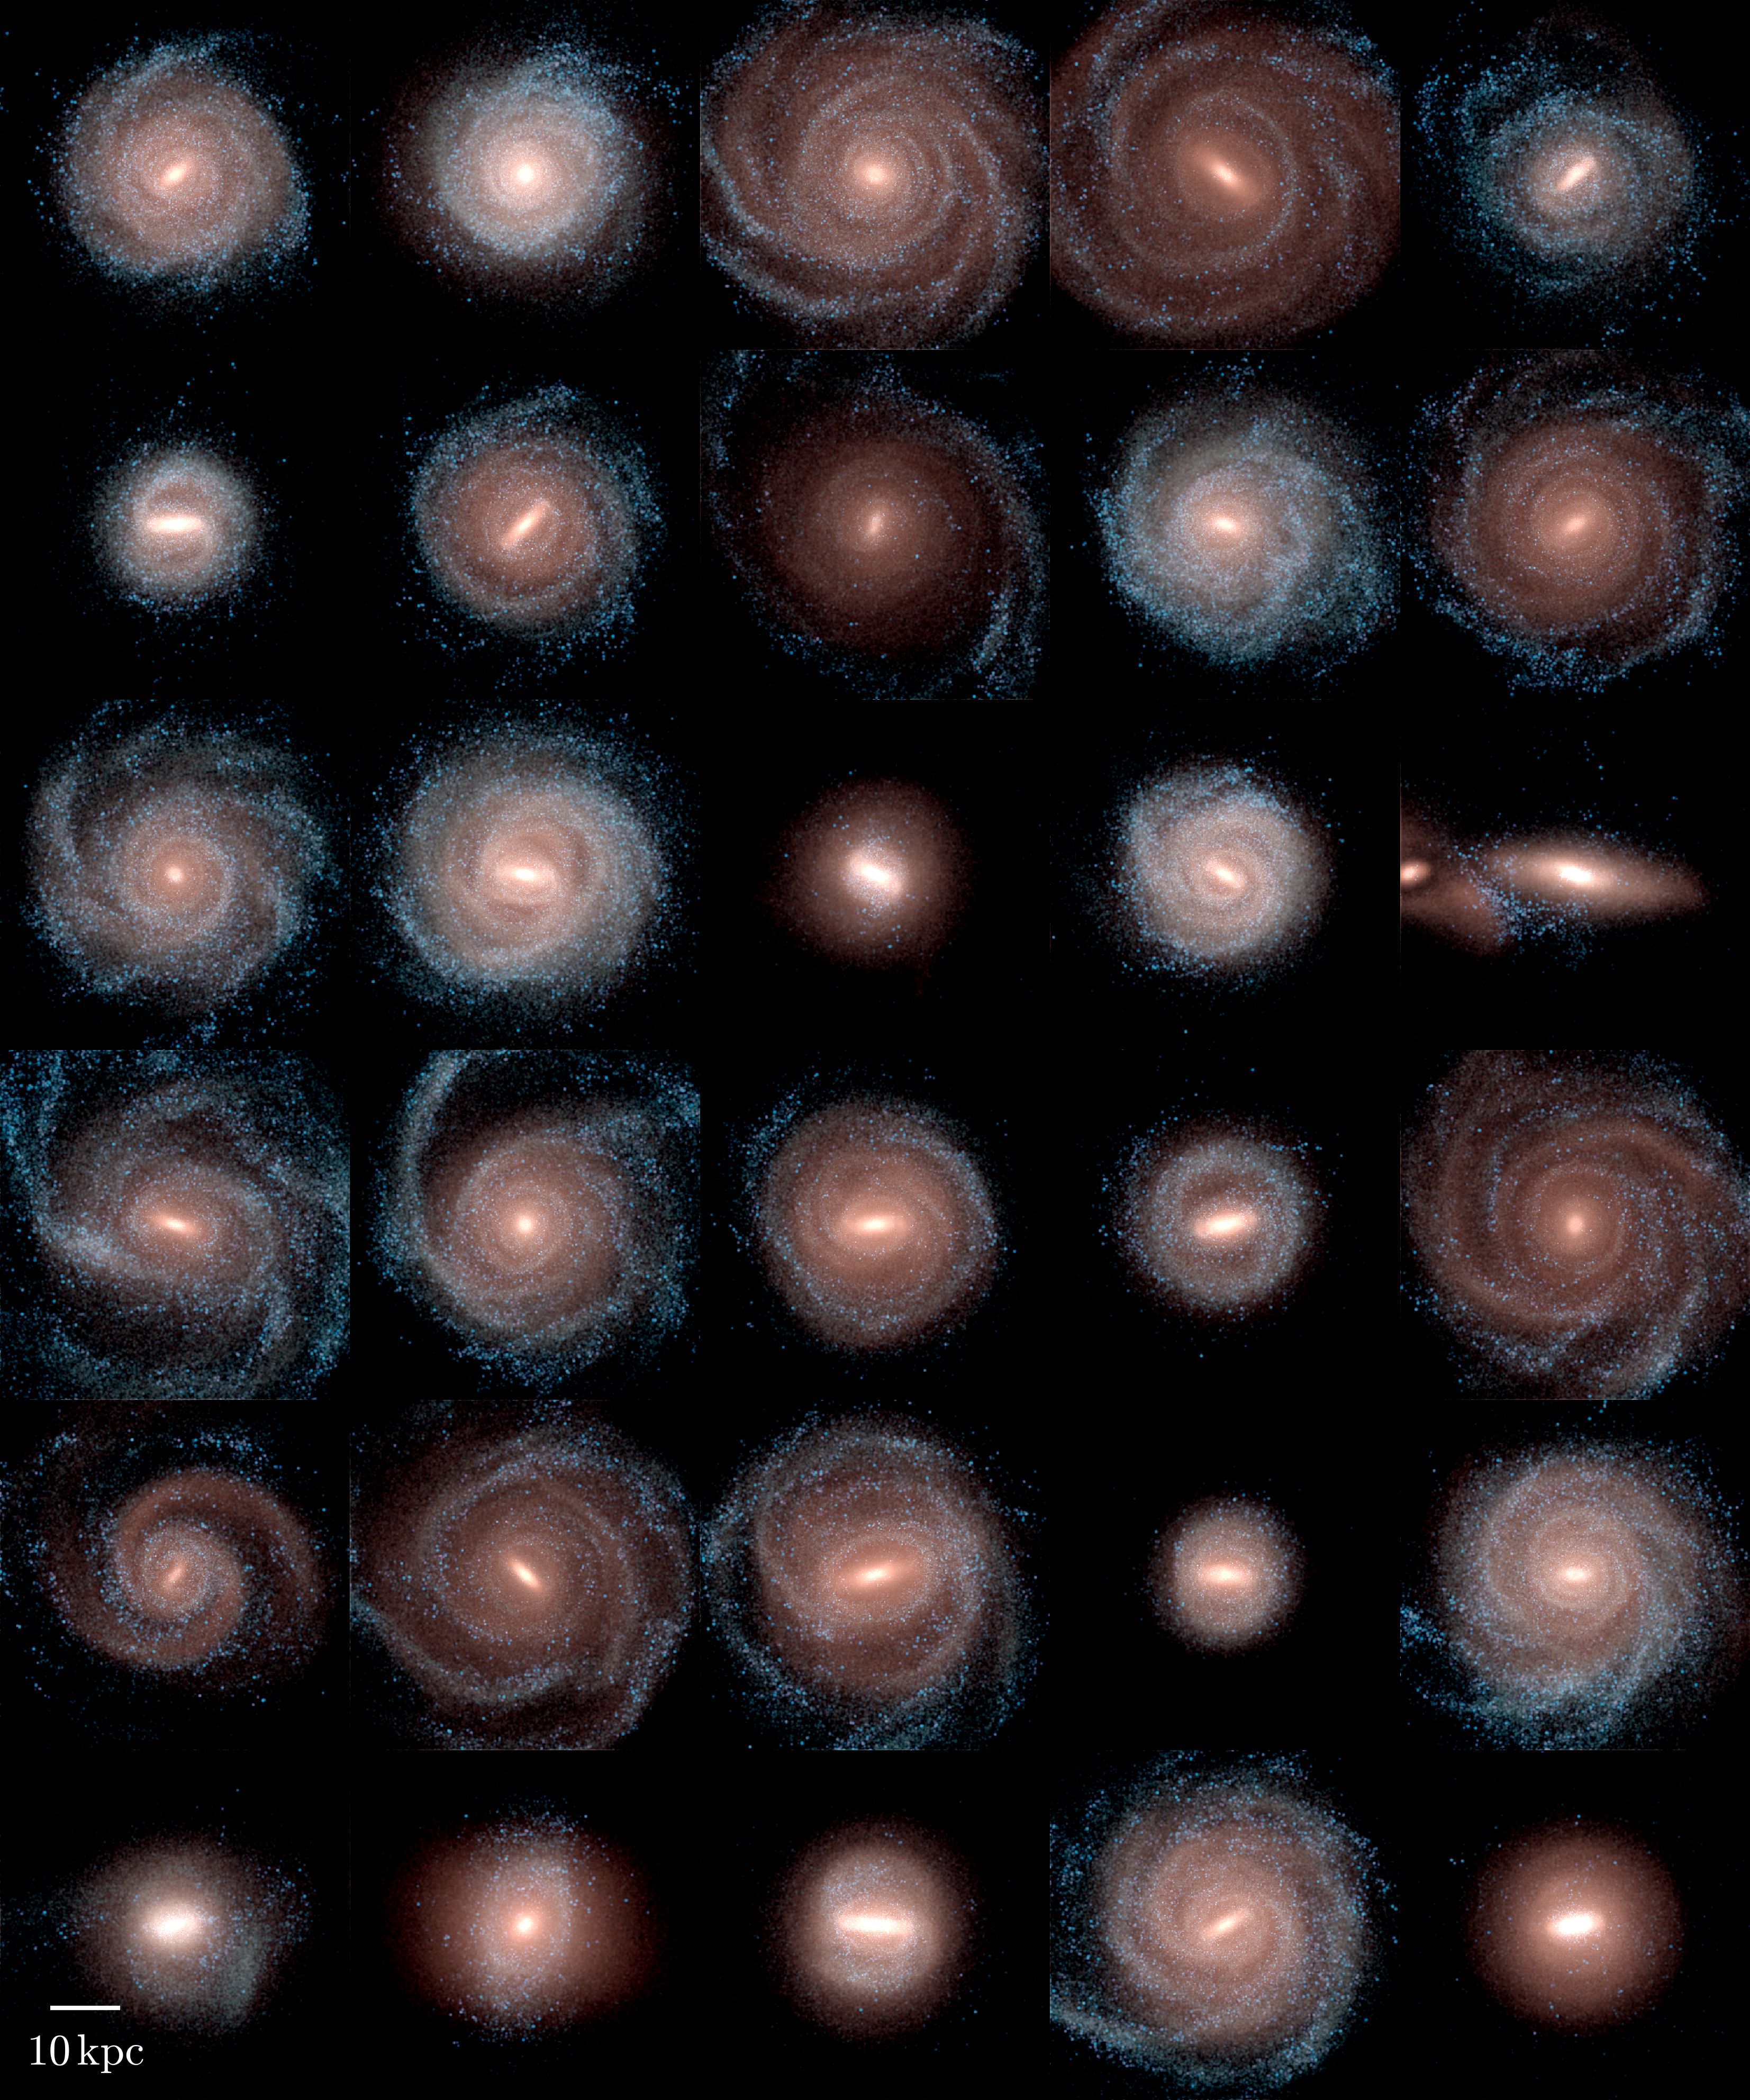
\includegraphics[width=0.8\textwidth]{./pics/Auriga.png}
    \caption{Set of 30 MW-like simulations, taken from http://auriga.h-its.org/}
    \label{fig:auriga}
\end{figure}

\section{Determining the halo shape}
Start saying that there is no unique method for determining the shape at a specific radius. In general this process is not trivial and there are many different(in theory) approaches which produce esentially the same results \cite{Vera-Ciro2010}. Mention that we are going to use method by Allgood et al 2006 \cite{AllGood2006} following the steps by Vera-Ciro2010.\\

The method starts with particles enclosed within a sphere, we calculate the reduced inertia tensor:

\begin{equation}
I_{ij} = \sum_k \frac{x_k^{(i)}x_k^{(j)}}{d^2_k},
\label{eq:inertia}
\end{equation}

that is not sufficient, which is why we recalculate until we achieve convergence. Present this recalculation explicitly with a scale transformation which intuitively means that our ellipse is becoming a sphere under that transformation which at the end is fully consistent (find better words).

\begin{align}
(x,y,z) &\rightarrow (x,y/q,z/s) \label{eq:scale}\\
q &=  b/a \nonumber \\
s &= c/a \nonumber ,
\end{align}

Specify that with this process we obtain both the radial profile and the historical shape by simply applying this method at different radii and redshifts.
 % Background Theory 

\chapter{Our results}

In this chapter we present the principal results of our work as well as some CDM-consistent phenomenology. First, we address convergence issues. Secondly, we study the relation of the axial ratios in terms of the radius. On third place, we show our results on the effect of baryons on the moulding of the shape. Finally, we study the evolution of the radial profile of the axial ratios. 

\section{Convergence Analysis}
One of the principal factors that may bias our study is the resolution of the simulations. Fortunately, Auriga simulations have level 3 and level 4 versions of 6 of the gaxies which we can use to analyze the numerical convergence of the results. Resolution may also affect our procedure for calculating halo shapes through the reduction of particles taken into account to calculate the inertia tensor.\\

To illustrate this, in figures \ref{fig:goodConvergence} we compare the halo shape at redshift 0 for level 3 and level 4 simulations. In this case, we can say that there is good convergence of the studied quantities with very small numerical bias. However, this is not the case for every simulated halo.\\

 By way of example, in figures \ref{fig:badConvergence} we present a halo where resolution significantly affected the shape. In this case, although the difference is not extreme, it requires attention and a more careful analysis.\\

\begin{figure}[!ht]
  \centering
  \subfloat[halo 6 DM]{\includegraphics[width=0.7\columnwidth]{./pics/Convergence/halo6_DM_3Vs4_good.png}}
  \hfill
  \subfloat[halo 27 MHD]{\includegraphics[width=0.7\columnwidth]{./pics/Convergence/halo27_MHD_3Vs4_good.png}}
  \caption{Level 3 (green) \& 4 (pink) radial profiles of axial ratios for halo 6 (DM) \& 21 (MHD). Here, it is clear that there is good agreement on the calculated quantities for both levels of resolution.}
  \label{fig:goodConvergence}
\end{figure}



\begin{figure}[!ht]
  \centering
  \subfloat[halo 16 DM]{\includegraphics[width=0.8\textwidth]{./pics/Convergence/halo21_DM_3Vs4_bad.png}}
  \hfill%\hspace{-0.5em}
  \subfloat[halo 23 MHD]{\includegraphics[width=0.8\textwidth]{./pics/Convergence/halo23_MHD_3Vs4_bad.png}}
  \caption{Level 3 (green) \& 4 (pink) radial profiles of axial ratios for halo 16 (DM) \& 23 (MHD). Here, axial ratios show slow convergence. }
  \label{fig:badConvergence}
\end{figure}


For instance, by simple inspection, we notice that there is no apparent systematic way in which resolution affects the halo shape. That is, sometimes the highly-resoluted halo appears rounder and other times it seems more triaxial. This is important for our study as we focus on the analysis of the triaxial properties of the halo. Incidentally, DM-only halos remain unchanged with the exemption of the radial regimes where the number of particles affects our shape-calculating method. However, for MHD simulations, the resolution of gas has a global influence over the axial ratios. We suspect this is caused by continuous exposition of particles to the resolution-sensible baryonic potential. Nevertheless, further calculations are needed to confirm the cause of these discrepancies.\\

Consequently, to rule out our shape method as a cause of these resolution differences, we decide to isolate the few-particle effect on our calculations. To do this, we randomly select DM particles from level 3 halos at $z=0$ to produce 10 samples of approximately the same size as level 4 simulations. We then calculate this few-particle effect, which we show in figures \ref{fig:convergence}. For each radius, we calculate the standard deviation of the sample shape and illustrate a 3-sigma range around the level 3 curve to compare with the respective level 4 shape values.\\  

From graphics on \ref{fig:convergence}, it is clear that the fractional difference is not actually significant and remains under $1\%$ for the majority of the radial profile. It becomes important for radii less than $1Kpc$ due to the lack of particles for approximating an elliptical shape. This is corroborated by the $3\sigma$ range, which also becomes evident around $1Kpc$. We deduce from this analysis that for radii bigger than $1Kpc$, the differences of level 3 and level 4 ellipses cannot be explained as an effect of the lack of particles. This is a confirmation that all kinds of matter are directly affected by resolution due to precision-sensitive events on the history of formation or because the numerical gravitational potential of matter continuously influences surrounding structures. Either way, even for the most resolution-biased cases, we can say that for the purposes of this study, convergence is achieved to a reasonable extent.\\  

\begin{figure}[!ht]
  \centering
  \subfloat[halo 24 MHD]{\includegraphics[width=0.7\columnwidth]{./pics/Convergence/rand_conv_halo24_DM.png}}
  \hfill
  \subfloat[halo 24 DM]{\includegraphics[width=0.7\columnwidth]{./pics/Convergence/rand_conv_halo24_MHD.png}}
  \caption{The few-particle effect on the axial ratios convergence for halo 24 (DM \& MHD). Here level4 curves (magenta) are compared to  the 3$\sigma$ range (clear blue) of the random-sampled curves from level3 (solid blue). We deduce from the fractional difference (green) that discrepancies at $r>>1$Kpc cannot be explained solely with the few-particle bias. }
  \label{fig:convergence}  
\end{figure}

\section{The radial dependence of axial ratios}
One of the our first results is related to the evolution of the DM halo shape in terms of the radius. We expect from previous work that the shape does not remain constant along the radius \cite{Vera-Ciro_et_al._2011}. Specifically, after some time, halos are gradually constructed from inner shells to outer shells through constant accretion of matter from cosmic structures \cite{Tormen_et_al._1997,Tormen_et_al._1998}. Inner shells tend to conserve their shape as a consequence of being shielded from the outside by Gauss law. Outer shells, on the other side, are continuously affected by the gravitational potential from the inside, which makes them prone to shifting orbits. This inner gravitational potential has a \textit{rounding} effect on the outerskirts. For this reason, we expect that halos are more triaxial on inner regions and more spherical at bigger radii. This effect has been corroborated on multiple cosmological simulations \cite{Frenk_et_al._1988,Dubinski_and_Carlberg_1991,Warren_et_al._1992,Cole_and_Lacey_1996,Hayashi_et_al._2007,Bett_et_al._2007,Vera-Ciro_et_al._2011}. \\


\begin{figure}[!ht]
  \centering
  \subfloat[halo 27 DM shape at small radius]{\includegraphics[width=0.5\columnwidth]{./pics/MHD_Vs_DM/level4_DM_halo_27_inner.png}}
  \hfill
  \subfloat[halo 27 DM shape at big radius]{\includegraphics[width=0.5\columnwidth]{./pics/MHD_Vs_DM/level4_DM_halo_27_outter.png}}
  \hfill
  \subfloat[halo 27 MHD shape at small radius]{\includegraphics[width=0.5\columnwidth]{./pics/MHD_Vs_DM/level4_MHD_halo_27_inner.png}}
  \hfill
  \subfloat[halo 27 MHD shape at big radius]{\includegraphics[width=0.5\columnwidth]{./pics/MHD_Vs_DM/level4_MHD_halo_27_outter.png}}
  \caption{DM density for inner (left) and outer (right) parts of the halo 27. We present both versions: DM (up) \& MHD (down). The horizontal and vertical axes are aligned to the major and medium semi-axes respectively. Here, it is evident that this halo is more spherical at bigger radii and more triaxial at the central parts. }
  \label{fig:slices}
\end{figure}

In figures \ref{fig:slices}, we present a halo in which this rounding effect is evident for both degrees of realism. However, to eliminate any possible cualitative bias, on figure \ref{fig:DM_MHD} we present a quantitative version of this effect. There, we include all axial ratios, which clearly become closer to 1 for bigger radii. Additionally, we include a quantification of the triaxiality, namely $T=\frac{1-b/a}{1-c/a}$.\\

 This measurement $T$ tends towards unity when the medium-to-major axis ratio becomes equal to the minor-to-major ratio, i.e. when the halo becomes prolate. When the medium axis is close to the major axis but not to the minor axis, $T$ tends to a null value, i.e. when the halo tends to an oblate shape. In these terms, halos are expected to be more prolate on the inside and more oblate on the outside. Even though the perfect spherical shape has a divergent/undefined $T$ value, prolate shapes are associated with triaxial characterizations and oblate shapes are identified as approximately spherical shapes. However, this can be confirmed on the triaxial $c/a$ Vs $b/a$ plane where we also demonstrate that this is in fact a global tendency for all halos.\\


\begin{figure}
\centering
{\includegraphics[width=1\columnwidth]{./pics/MHD_Vs_DM/level4_halo_27_DM_Vs_MHD.png}}
\caption{Radial profile for axial ratios and triaxiality parameter $T=\frac{1-b/a}{1-c/a}$ from halo 27. This halo has a clear radial tendence towards sphericity (for bigger radii), which can be confirmed with the triaxiality parameter. }
\label{fig:DM_MHD}
\end{figure} 


In figure \ref{fig:Triaxiality_Inner_Outer}, we show the axial ratios on the plane $c/a Vs b/a$. There, each dot labeled by radius represents a specific shape. In this plane, oblate halos are represented by the vertical line $x = 1$, prolate halos are identified on the identity line and spheres are exactly the point $(1,1)$. This gives us a broader idea of the evolution of the shape. The tendency is clear for halos to get rounder with increasing radius. In fact, the difference in shape clear enough that it is possible to identify groups in case the radius label is lost.\\

\begin{figure}[!ht]
  \centering
  \subfloat[Level4 MHD Vs DM at inner regions]{\includegraphics[width=0.7\columnwidth]{./pics/Triaxial_Plane/Triaxiality_Inner_lvl4.png}}
  \hfill
  \subfloat[Level4 MHD Vs DM at outter regions]{\includegraphics[width=0.7\columnwidth]{./pics/Triaxial_Plane/Triaxiality_Outter_lvl4.png}}
  \hfill
  \caption{Axial ratios as shown on $c/a$ Vs $b/a$. Each dot represents a halo shape at some radius. Some observational constraints are plotted alongside our results. Here, dots are clustered, proving the general tendence of halos to get rounder on the outer parts. }
  \label{fig:Triaxiality_Inner_Outer}
\end{figure}


\subsection{The effect of gas on the halo shape}
We have simultaneously corroborated the rounding effect of radius on the halo shape from DM-only and MHD simulations. However, from the parallel presentation of results from MHD and DM simulations, it is noticeable that MHD halos are in general more spherical than DM halos, which is to be expected \cite{Barnes_and_Hernquist_1996,Springel_et_al._2004,Bryan_et_al._2013}.\\

 Unlike DM, gas collapses and generates disks which are much denser than the DM structures. This amplifies the effect of the gravitational potential and, if we apply the same logic, we would expect that the inner regions of the halo are more spherical where there is presence of gas. We expect the same for outter regions but this effect is predicted to be more significant due to a continuous effect of the gravitational potential of inner shells.\\

For instance, recurring again to the figures \ref{fig:slices}, now comparing the graphics vertically, the rounding effect of visible matter is clear. For a more cuantitative illustration of this, we can reffer to figure \ref{fig:DM_MHD}. \\
\begin{figure}[!ht]
  \centering
  \subfloat[Level4 DM inner Vs outer regions]{\includegraphics[width=0.7\columnwidth]{./pics/Triaxial_Plane/Triaxiality_DM_lvl4.png}}
  \hfill
  \subfloat[Level4 MHD inner Vs outter regions]{\includegraphics[width=0.7\columnwidth]{./pics/Triaxial_Plane/Triaxiality_MHD_lvl4.png}}
  \hfill
  \caption{General tendence on the triaxial plane $c/a$ Vs $b/a$. Some observational constraints are plotted alongside our results}
  \label{fig:Triaxiality_DM_MHD}
\end{figure}

Although from previous pictures it is evident that the presence of gas affects the halo shape making it rounder, it is not clear that this effect is amplified for bigger radii. To confirm this, we reccurr again to triaxiality plane on \ref{fig:Triaxiality_DM_MHD}, where this tendency becomes evident.\\


So far, our results are in accordance with previous work. Nonetheless, in the specific case of MW-like galaxy simulations, we have confirmed the expected tendence in an unprecedented statistically significant sample of 30 galaxies form Auriga, compared to the 4-sample galaxies from the previous state-of-the-art Aquarius simulations. Moreover, we confirmed that these results are sustained for the specific case of novel MHD MW-like galaxy simulations where we could analyze effect of gas.\\

\section{Historical shape}
Taking into account the previous fenomenology for halo formation, it is possible to extend 
its reach for the analysis of the historical evolution of the halo shape.\\

 Recalling that inner shells of the halo are isolated from the gravitational effect of outer shells, the only significant source of disruption in time of this radial regime are external structures that perform some torque on them. Outter shells must feel this source of deformation too in addition to the effect from the inner gravitational potential. Consequently, we expect a systematic change on the halo shape with time, which becomes more significant for bigger radii.\\
 
Major events like mergers, may completely disturb a galaxy shapes and erase any memory of it. However, from $z~1$ onwards, these events are very rare \cite{Tormen_et_al._1998} and we expect that any source of disruption is weak and is reduced to the previously mentioned factors. These sources of potential asymmetries influence DM particles towards more spherical orbits \cite{Debattista_et_al._2008}. \\  

\begin{figure}[!ht]
  \centering
  \subfloat[halo 16 DM]{\includegraphics[width=0.7\columnwidth]{./pics/Redshift/halo_16_level3_DM_Z.png}}
  \hfill
  \subfloat[halo 16 MHD]{\includegraphics[width=0.7\columnwidth]{./pics/Redshift/halo_16_level3_MHD_Z.png}}
  \caption{Radial profile (comoving) of axial ratios for halo 16 in terms of redshift (color). This halo maintains its shape until $z\approx 1$ obviating the systematic rounding effect in time from asymmetric potentials. }
  \label{fig:RedshiftGood}
\end{figure}

In figures \ref{fig:RedshiftGood} we present the evolution of the radial profile of the shape of a halo that managed to conserve its integrity until $z \approx 1$. In this case, we show our results in terms of the comoving coordinates to obviate the scale factor and make these profiles comparable. The halo becomes systematically more spherical as it evolves in time, being this effect more relevant for $r>50Kpc$.\\

In figures \label{fig:RedshiftDMbad} we present a special case of a halo that was perturbed at some time around $z\approx 0.5$. It is specially evident because of the discontinuity caused in the radial profile and the large differences in the virial radii. In figure \ref{fig:RedshiftSnaps}, we confirm that the source of this disruption is a moderate sized infalling subhalo around $z\approx 0.5$.  \\  


\begin{figure}[!ht]
  \centering
  \subfloat[halo 21 DM]{\includegraphics[width=0.7\columnwidth]{./pics/Redshift/halo_21_level3_DM_Z.png}}
  \hfill
  \subfloat[halo 21 MHD]{\includegraphics[width=0.7\columnwidth]{./pics/Redshift/halo_21_level3_MHD_Z.png}}
  \caption{Radial profile (comoving) of axial ratios for halo 21 in terms of redshift (color). This halo is disrupted around $z \approx 0.5$ which results in a certain loss of its shape memory.}
  \label{fig:RedshiftBad}
\end{figure}

Now, these results compare radial profiles in comoving coordinates, but in real life we have physical coordinates. In this order of ideas, we can state this preservation of the shape (obviating the rounding effect) without recurring to comoving comparisons.\\

In this case, consider a physical radius $R$ that is well-defined for each redshit. It is the radius at which we are going to perform our historical measurements. For practical purposes let us take, for example, the virial radius at each redshift. Then, as halos are continuosly accreting matter, the virial radius will be in general smaller (in comoving, just as means of comparison) for higher redshifts. This means we are effectively sampling the shape for smaller radii at higher redshifts. Taking into account that the halo shape is well conserved in time, we expect that the historical profile of the axial ratios at a certain physical radius is correlated to the radial profile of the same halo at the present time. \\

To illustrate this, in figures \ref{fig:RedshiftDMTriax16,fig:RedshiftDMTriax21} we present the historical and radial profiles of the previously analyzed halo shapes. For the halo that maintained a consistent shape during time, there is a clear correlation between the historical and radial profiles, both clearly tending to more spherical shapes at lower redshifts and bigger radii. In the case of the halo that had a major disrupting event, this correlation is not clear as an evidence of memory loss by the massive infalling material.\\  

%\begin{verbatim}
\begin{figure}[!ht]
  \centering
  \subfloat[halo 16 MHD]{\includegraphics[width=0.7\columnwidth]{./pics/Redshift/halo_16_level3_MHD_Z_Triax.png}\label{fig:RedshiftDMTriax16}}
  \hfill
  \subfloat[halo 21 MHD]{\includegraphics[width=0.7\columnwidth]{./pics/Redshift/halo_21_level3_MHD_Z_Triax.png}\label{fig:RedshiftDMTriax21}}
  \caption{Historic shape (color dots) Vs actual radial shape (solid black line) on the Triaxiality plane. Each colored dot represents a calculated shape at R Mean 200, for each redshift. It is clear that halos with memory, unlike disrupted halos, have correlation between their historical and radial profiles.}
\end{figure}
%\end{verbatim}







 
 % Experimental Setup

\chapter{Conclusions}

In this work we use Allgood's method for shape calculation \cite{Allgood_et_al._2006} on the 30-sized set of DM-only and MHD MW-like simulations from the Auriga project to verify the results obtained by Vera-Ciro et al. 2011 about the shape of DM halos from Aquarius simulations and obtain more insight about how DM halos look on MW-like simulations. Auriga includes consistent models for energetic and accretion feedback from stars and Black Holes and the unique inclusion of magnetic fields. These models worked over a significant set of 30 galaxies evolved with the Arepo code, which solves the principal problems of the previous Computational Fluid Dynamys paradigms. All these properties make of Auriga one of the most advanced and precise simulations in actuality.\\ 

Our work is motivated by various factors. On one hand, obtaining insight on the halo shape of full-physics MW-like simulations may be applied to the improvement of constraints on the DM density field of our MW. This would result in a better comprehension of the behaviour and nature of DM itself. On the other hand, the novelty of gas models in these simulations makes them unique for the understanding on how the presence of visible matter affects the axial ratios of DM halos. Given the vast work on DM-only simulations, our results could be applied to make more realistic conclusions on these previous studies. Finally, the unique significant sample of 30 high-resolution galaxies from Auriga simulations makes our results statistically-supported.\\  

Taking this into account, we verify that, at $z=0$, DM halos from DM-only and MHD simulations are more oblate/spherical on outer regions and more prolate/triaxial on inner parts. We corroborate this effect in different manners, by obtaining the radial profile of the axial ratios, calculating a triaxiality indicator $T$ and presenting our results on the triaxial plane. Although our results were expected from the work on various cosmological simulations \cite{Frenk_et_al._1988,Dubinski_and_Carlberg_1991,Warren_et_al._1992,Cole_and_Lacey_1996,Hayashi_et_al._2007,Bett_et_al._2007,Vera-Ciro_et_al._2011}, our study is supported with an unprecedented sample of 30 level 4 resolution MW-like simulated galaxies.\\

Taking advantage of the parallel outcome of DM-only and MHD versions of the same galaxies on Auriga, we compare both versions to analyze the effect of the presence of gas on the shape of the DM halos. We find that gas affects the shape at all radii by makin the halo more spherical. Furthermore, we demonstrate that this rounding effect is more prominent on the outer regions of the halo. Although the general rounding effect due to the presence of matter is expected taking into account previous studies on cosmological simulations \cite{Barnes_and_Hernquist_1996,Springel_et_al._2004,Bryan_et_al._2013}, our results are in conflict with precedent work on the strength of this effect in terms of radius \cite{Bryan_et_al._2013}. Usually, it is found that the rounding of halos is more evident on inner parts than on the outerskirts.\\

Vera-Ciro et al. deduced by inspection and showed that there is a correlation between the radial profile of the halo's axial ratios and the historical evolution at a determined radius. We corroborate this fact for DM-only simulations and show the reason for this correlation by calculating the radial shapes at comoving coordinates. We discover that the shape remains more or less unchanged in time once we account for the continuous rounding effect which is shown to be more prominent on the outerskirts of the halo, due to the continuous exposure to the inner gravitational potential. This is consistent with our results on the strength of the rounding effect of gas, which is also more intense for bigger radii.\\

We conclude our study by stating some interesting questions and proposing further studies on this matter.\\

First, our results are in general supported by previous works on cosmological simulations, with the exemption of the strength of the rounding effect of gas. In this sense it is of special interest to identify the causes of these discrepancies. We suspect that the principal source of these discrepancies may lie on the differing galaxy-formation models, the performance of the studies on different kinds of simulations and numerical effects of scattering. Previous work showed that the feedback efficiency diminishes the rouding effect by preventing matter to collapse at the center of the galaxy \cite{Bryan_et_al._2013}. In the case of Auriga simulations, to produce realistic MW-like disks, AGN feedback plays an important role in limiting the formation of stronge bulges \cite{auriga}, which diminishes the strength of the effect based on conclusions from previous work. However, previous works are not limited to the study of MW-like galaxies but study galaxies in the general cosmological context and inconsistencies may be due to specific effects of MW-like galaxies. Additionally, the rounding effect may be affected by resolution of previous work simulations. Here, we find that there is indeed a bigger resolution effect on MHD simulations due to the presence of gas, which may also contribute to these discrepancies. Nontheless, to confirm the causes of this conflic, further work must be performed.\\

Secondly, this work may be extended to the analysis of the impact of environmental structures on the shape of the DM halo. Here, following the work of Vera-Ciro et al. 2011, we must also analyze the relation of shapes with angular momentum and the specific orientation of the principal axes of the halo with respect to those determined by cosmic structures like fillaments. This could shed light on the effect of external structures on the DM halo shape, giving a more complete picture of how the the DM halos are shaped through history.\\


Finally, we could make use of the exeptional number of simulated galaxies to address statistical problems. For example, we could corroborate and improve theoretical models that predict the response of DM halos to the presence of matter, such as adiabatic contractions \cite{Gnedin_et_al._2004}. Adiabatic contractions arise from the assumption that the mass of gass increases at the center of the halo so slowly that we can consider that at any time, DM particles reach a stable orbit. Making use of adiabatic invariants, one could obtain a relation between the DM halo density and the gas density. This would support the advanced work on DM-only simulations by making them more observationally comparable by including the effects of gas, as well as making predictions of DM halos from the observed content of gas.\\




 
 
 % Experiment 1

%\input{Chapters/Chapter5} % Experiment 2

%\input{Chapters/Chapter6} % Results and Discussion

%\input{Chapters/Chapter7} % Conclusion

%% ----------------------------------------------------------------
% Now begin the Appendices, including them as separate files

\addtocontents{toc}{\vspace{2em}} % Add a gap in the Contents, for aesthetics

\appendix % Cue to tell LaTeX that the following 'chapters' are Appendices

%\input{Appendices/AppendixA}	% Appendix Title

%\input{Appendices/AppendixB} % Appendix Title

%\input{Appendices/AppendixC} % Appendix Title

\addtocontents{toc}{\vspace{2em}}  % Add a gap in the Contents, for aesthetics
\backmatter

%% ----------------------------------------------------------------
\label{Bibliography}
\lhead{\emph{Bibliography}}  % Change the left side page header to "Bibliography"
\bibliographystyle{unsrtnat}  % Use the "unsrtnat" BibTeX style for formatting the Bibliography
\bibliography{Bibliography}  % The references (bibliography) information are stored in the file named "Bibliography.bib"

\end{document}  % The End
%% ----------------------------------------------------------------
